Los tipos de interfaces podríamos definirlos de la siguiente forma:

\subsection{Control automatizado}

Este tipo de interfaces está enfocada a poder controlar dispositivos
especializados de una manera sencilla, para ayudar a los operadores
en su labor.

Un buen ejemplo es un software llamado \emph{Hevelius}~\cite{hevelius},
el cual es una aplicación que, utilizando un sistema de control
de telescopios distribuidos, utilizando un framework de desarrollo
llamado ALMA Common Software (ACS)~\cite{acs},
permite el control de un Telescopio real o un telescopio en un ambiente
simulado.

La idea principal es poder generar un entorno simple~\ref{fig:hevelius},
para tanto astrónomos aficionados como profesionales,
en el cual se representan conceptos básicos del control de telescopios,
pudiendo ser un buen acercamiento al mundo de la astronomía.

\begin{figure}[!htb]
\begin{center}
    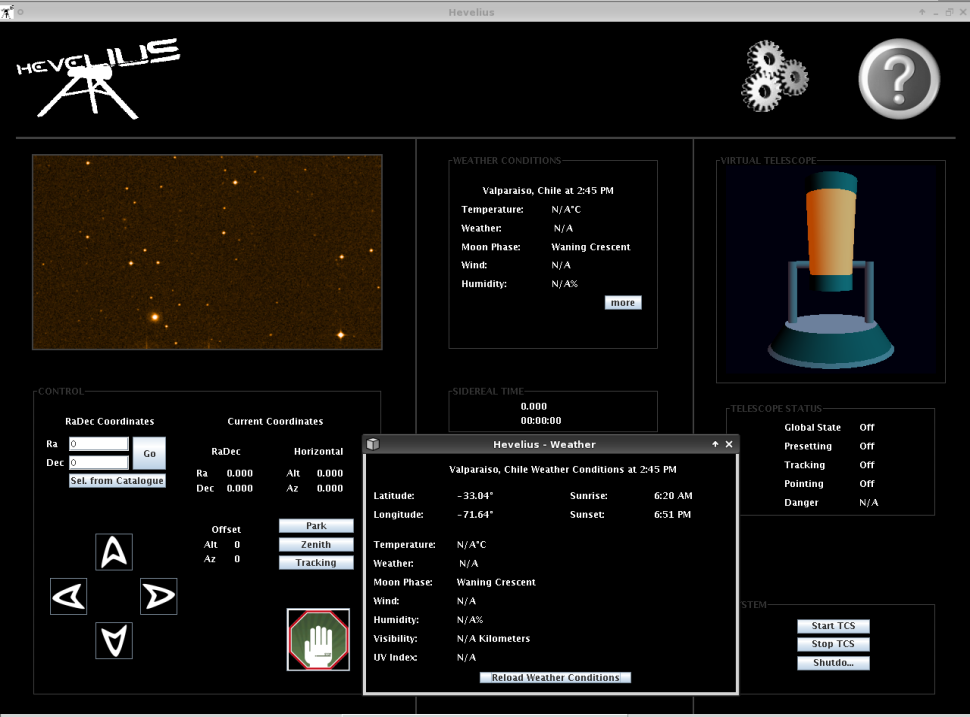
\includegraphics[width=0.4\textwidth]{img/hevelius}
    \caption{\emph{Hevelius}, ventana principal}
    \label{fig:hevelius}
\end{center}
\end{figure}

La interfaz posee tres secciones principales,

\begin{itemize}
    \item Visualización en tiempo real del cielo, la cual
        consiste en la parte principal  del programa,
        al ser un elemento que debe ser modificado en tiempo real
        a medida que el telescopio se mueva.
    \item Control del telescopio, los que permiten poder
        mover ya sea manualmente el telescopio, o manualmente
        ingresando la información en radianes, o seleccionar
        de un catalogo una posición determinada.
    \item Estado del telescopio y elementos externos,
        de los cuales se pueden observar condiciones climáticas,
        las cuales son muy importantes a la hora de realizar
        una observación.
\end{itemize}

La interfaz es bastante simple,
salvo que hay información que quizás no sea necesaria
desplegar todo el tiempo, o mejor dicho,
que podrían ser agrupados de mejor forma,
debido a que la imagen real del cielo tiene
menos de un 25\% del tamaño de la interfaz.

\subsection{Análisis de datos}

Otro enfoque para interfaces astronómicas, son las cuales nos permiten
poder realizar dos tareas
principales:
\begin{itemize}
    \item Obtener datos de un dispositivo o sistema (Sampling).
    \item Manipular y/o analizar los datos.
\end{itemize}

Un ejemplo que clarifica este enfoque es la herramienta llamada
\emph{Sampling System GUI (SSG)}~\cite{ssg}, la cual provee una buena
aproximación de como utilizar la API del subsistema de ACS~\cite{acs} llamado
\emph{Sampling System}~\cite{acssamp}, para poder obtener datos y
representarlos de forma gráfica~\ref{fig:ssg}, implementando una interfaz básica,
siendo su objetivo obtener la información de distintas propiedades
de dispositivos en una antena radioastronómica.

Las interfaz provee distintas opciones para realizar este proceso,
las cuales son:
\begin{itemize}
    \item Obtener datos en un periodo de tiempo,
    \item Obtener información a diferentes secuencias,
    \item Obtener información de varias propiedades en la misma ventana,
    \item Guardar datos en archivos CSV, entre otras.
\end{itemize}

\begin{figure}[!htb]
    \centering
    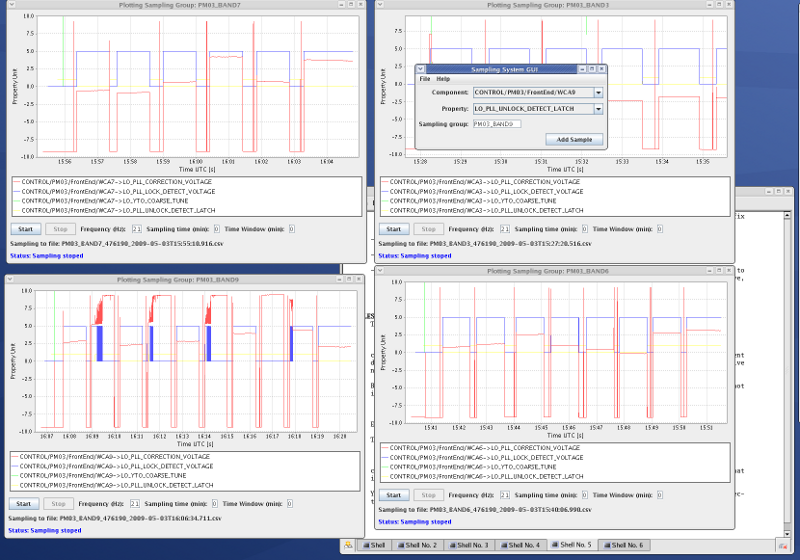
\includegraphics[width=0.4\textwidth]{img/ssg}
    \caption{\emph{Sampling System GUI}, gráficos más ventana principal}
    \label{fig:ssg}
\end{figure}

Es en esta temática, donde es muy importante realizar una elección adecuada de
dos aspectos principales, el lenguaje de programación y la biblioteca
gráfica para realizar el procedimiento de despliegue de información,
sobre todo si se trata de un sistema que recolecte información
en tiempo real.

Una investigación que aborda este problema, es el trabajo de Maureira et al~\cite{hpg}
donde presentan un estudio sobre la correcta elección entre lenguajes de programación,
(Python, C++ y Java) y algunas bibliotecas gráficas, en las cuales se definen variados
temas importantes, como por ejemplo, la simplicidad del código para poder mantenerlo,
y la cantidad de elementos que nos favorecen el trabajo a la hora de poder desarrollar
una interfaz gráfica.

\subsection{Configuraciones de sistemas}

En grandes proyectos, con una gran cantidad de variables y sistemas, que se relacionan
unos con otras, una simple acción o accidente puede provocar una cadena de reacciones
debido a la naturaleza del sistema.

Por ejemplo, si un cable de red que conecta dos computadores de pronto se corta,
todas las aplicaciones que utilizan dicha conexión fallarán, lo que provocará
que otras aplicaciones también fallen, y así sucesivamente.

¿Que problema más profundo puede ovacionar esto?
de que todos los errores de las aplicaciones y/o dispositivos pueden crear
una gran confusión al momento de buscar el problema.

Aquí una interfaz gráfica~\ref{fig:acg} llamada Alarms Configuration GUI (ACG)~\cite{acg},
la cual se basa en manipular todas las señales y configuraciones del ACS Alarm System (AS)~\cite{as},
que está a cargo de definir y reportar todas las fallas de un sistema que utilice
el framework ACS como base.

La idea de esta interfaz además es poder realizar todo este mecanismo de configuraciones,
mediante variados archivos XML, los cuales poseen la característica primordial de ser
validados mediante archivos XSD.

\begin{figure}[!htb]
    \centering
    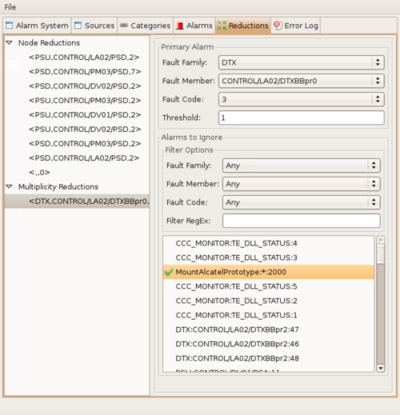
\includegraphics[width=0.4\textwidth]{img/acg}
    \caption{\emph{Alarms Configuration GUI}, ventana de propiedades}
    \label{fig:acg}
\end{figure}

La interfaz es un claro ejemplo,
de una problemática muy habitual al momento
de querer realizar programas para configurar variadas opciones de sistemas,
las cuales de mala forma suelen llenar una vista principal
de demasiadas opciones, volviendo la interfaz en algo poco eficiente,
pero en este caso, se han organizado distintas vistas,
para poder realizar las configuraciones y revisar los estados
de una forma mas ordenadas, lo que se pudo llevar a cabo utilizando
pestañas.

\subsection{Observatorios virtuales y planetarios}

El concepto de un observatorio virtual tiene relación a un conjunto de archivos
con datos astronómicos, interactivos y que utilizan distintas
herramientas de software, en este caso, interfaces gráficas, las cuales
mediante una conexión directa con los servidores donde se encuentra
la información, pueden generar un ambiente real de trabajo,
el cual puede ser utilizado por científicos en distintos lugares del mundo.

En palabras simples, podríamos decir que un observatorio virtual es un conjunto
de centros de datos, los cuales son colecciones de datos astronómicos,
los que están apoyados por herramientas de software para realizar
cálculo científico.

La idea detrás de las interfaces gráficas consiste,
en poder automatizar distintos procesos astronómicos,
como cálculos de coordenadas, aplicar filtros, búsqueda
de datos, recuperación de información, etc.

Por otro lado sabemos que un planetario es un lugar ideado
para poder desplegar sucesos o elementos astronómicos,
pudiendo observar una recreación de todo el espacio,
ya sean planetas, estrellas, etc, pero el concepto
no es sólo un lugar físico, como un museo, sino que también
sirven aplicaciones gráficas que cumplen la misma función,
los cuales se esmeran en poder simular la posición
del cielo, estrellas, galaxias, constelaciones, etc.

A continuación se detallan algunas aplicaciones que siguen la lógica
de los dos conceptos descritos anteriormente.

\subsubsection{KStars}

Esta aplicación gráfica, está diseñada como parte del módulo
de educación del proyecto KDE~\cite{kde}.
Su idea principal es poder ofrecer una simulación
del cielo nocturno, la cual contiene información
de estrellas, constelaciones, nebulosas, galaxias, planetas, etc.

La simulación se basa en poder observar el cielo desde cualquier
ubicación en el mundo, a cualquier hora, lo cual es una herramienta
muy útil para astrónomos amateurs, debido a que con \emph{KStars}
uno puede buscar las constelaciones en mi ubicación actual
para poder enfocarlas con algún telescopio amateur.

La interfaz que provee~\ref{fig:kstars2} es bastante intuitiva y flexible,
debido a que se conforma de un menú superior, con accesos directos 
a las opciones más importantes, las cuales permiten poder configurar
a gusto las capas que se despliegan, las que pueden ser:

\begin{itemize}
    \item Estrellas,
    \item Objetos celestes,
    \item Objetos del sistema solar,
    \item Constelaciones,
    \item etc.
\end{itemize}

y además un menú estándar de cualquier aplicación KDE.

Al comienzo del programa, existe un wizard~\ref{fig:kstars1} que permite al usuario
seleccionar la posición en el mundo en que se encuentra,
ya sea ingresando manualmente longitud y latitud, o seleccionando
la ciudad de una lista.

Por otro lado el plano estelar tiene opciones de zoom, llevados a cabo
con el mouse, entregando al usuario la facilidad de buscar e identificar objetos
en el cielo.

\emph{KStars} contiene variados catálogos de la información
de las estrellas en el cielo, entregando al usuario la posibilidad
de descargar material externo, como imágenes especializadas,
tipos especiales de nebulosa y otros catálogos de estrellas.

Finalmente \emph{KStars} está pensado para dos tipos de públicos,
astrónomos amateurs y educadores/estudiantes, siendo este último
un público objetivo que puede sin problema, ajustar velocidades
de ciertas simulaciones de fenómenos, realizar cálculo astrales,
optar a cursos en línea de información astronómica y poder
obtener imágenes reales de bases de datos mundiales.

\begin{figure}[!htb]
    \centering
    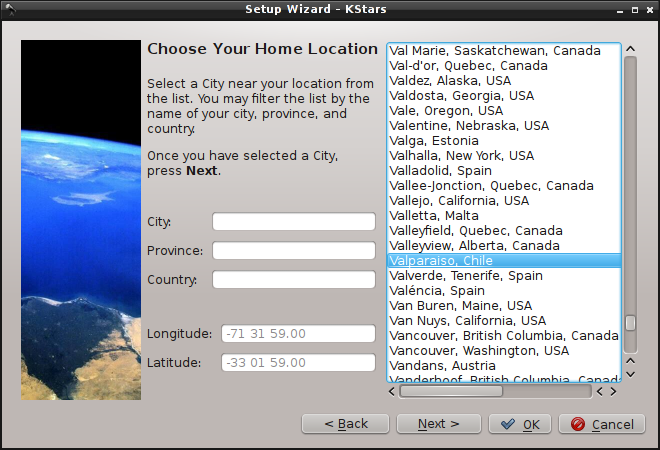
\includegraphics[width=0.3\textwidth]{img/kstars1}
    \caption{\emph{KStarts}, wizard de configuración}
    \label{fig:kstars1}
\end{figure}

\begin{figure}[!htb]
    \centering
    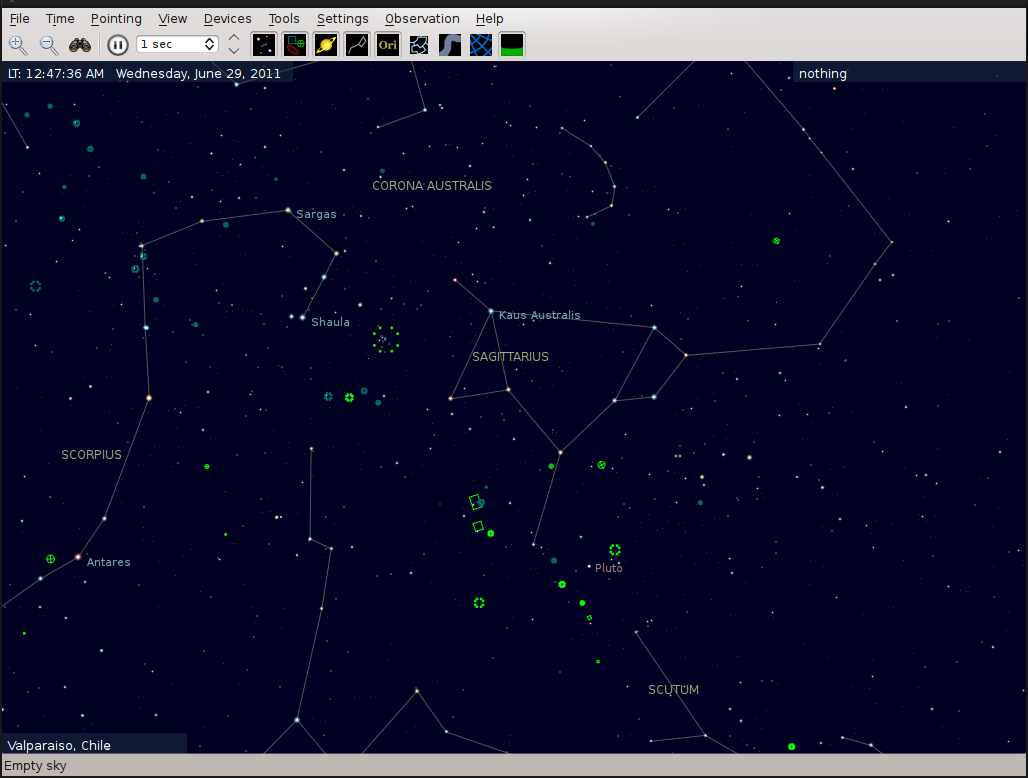
\includegraphics[width=0.5\textwidth]{img/kstars2}
    \caption{\emph{KStarts}, ventana principal}
    \label{fig:kstars2}
\end{figure}



\subsubsection{GCX}

Esta herramienta está enfocada a el procesamiento de imágenes astronómicas
y reducción de datos de la misma naturaleza, centrando su objetivo en proveer
una interfaz simple.

\emph{GCX} provee diferentes funcionalidades para realizar fotometría
con cámaras CCD, utilizando identificación de objetos celestes,
utilizando un sistema llamado WCS. Por otro lado, respecto al procesamiento
de imágenes, permite al usuario utilizar funciones para tratar dichas
imágenes, de manera de por ejemplo, eliminar ruido, alinear con respecto
a otros objetos, intensidad de colores, etc.

Una de las característica importantes de \emph{GCX} es sin lugar a dudas,
el control de cámaras CCD y telescopios amateur, las cuales
permiten al usuario ingresar la ruta a algún script que permita
realizar una rutina de observación, de la cual, provee la funcionalidad
de ayudar astrónomos amateurs a poder apuntar correctamente el telescopio
a un lugar determinado en el cielo, tarea principal para realizar
una buena observación.

Al proveer información de catálogos internacionales,
asegura un funcionamiento con bastante precisión,
tarea que no es sencilla a la hora de realizar
una interfaz que interpreta información precisa.

La interfaz~\ref{fig:gcx}, a modo de diseño es bastante simple y
poco llamativa a la vista
del usuario, pues no utiliza ninguna biblioteca externa para poder
generarla, sólo las que provee Xorg.
El único menú superior contiene todas las opciones
necesarias para poder trabajar con las imágenes
y el control de dispositivos, pero no ofrece
ningún wizard de configuración o algún mensaje que advierta
al usuario, que se deben descargar por separado las imágenes
en formato \emph{fit} o que se deben configurar los servidores
para obtener imágenes de un catalogo.

\begin{figure}[!htb]
    \centering
    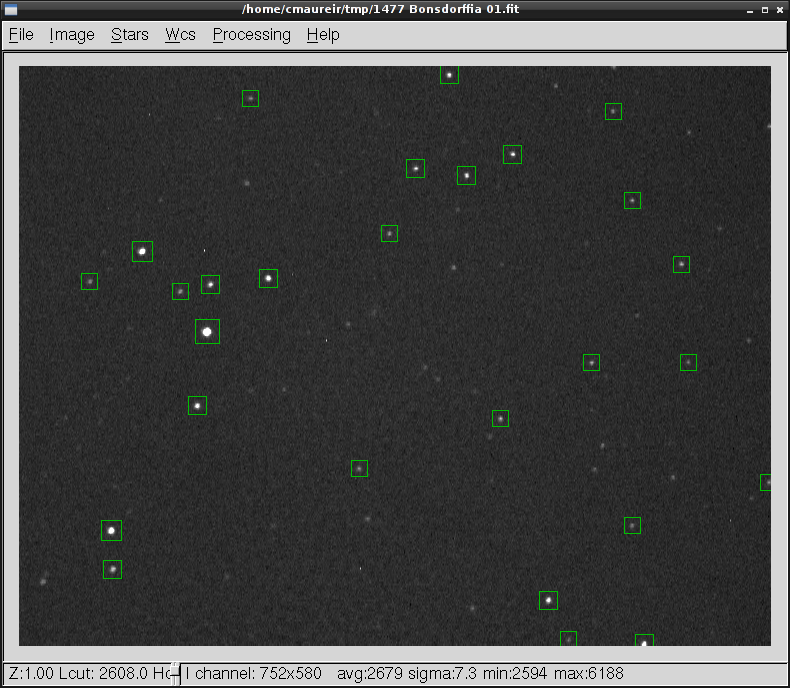
\includegraphics[width=0.5\textwidth]{img/gcx}
    \caption{\emph{GCX}, ventana principal con una imagen en formato $fit$ cargada.}
    \label{fig:gcx}
\end{figure}

\subsubsection{Celestia}

La presente aplicación, tiene como objetivo principal la simulación
del espacio, para poder visualizar el universo de una forma
cercana a la real, en tres dimensiones.

Al momento de seleccionar cualquier punto en el espacio,
la aplicación mostrará aparte de la aproximación visual
de cómo se debería ver, desplegará información detallada,
de la posición, la cual será útil para astrónomos amateurs,
para poder posicionar correctamente un telescopio.

El objetivo principal de \emph{Celestia}
es poder transformar la experiencia de un observatorio virtual
en algo inolvidable, y lo consigue por el dinamismo de los recorridos
virtuales.

Otra características importante, es que la aplicación
no sólo permite poder navegar en el sistema solar,
sino que además permite viajar a lugares
muy distantes en comparación a nuestra galaxia.

\emph{Celestia} provee una interfaz llamativa~\ref{fig:celestia},
basada en la biblioteca gráfica GTX, la cual consiste en una única ventana,
en la cual despliega la simulación de la galaxia,
teniendo en su parte superior un menú bastante simple de comprender
a la hora de buscar alguna opción determinada,
como cargar una rutina, buscar posiciones de planetas, etc.

Posee la buena idea de poder
brindar al usuario una ruta por distintas localidades,
desplegando información astronómica útil,
acerca de planetas, distancias, etc,
lo cual puede ser un punto a favor si queremos
enfocar estar interfaz a nivel educacional.

\begin{figure}[!htb]
    \centering
    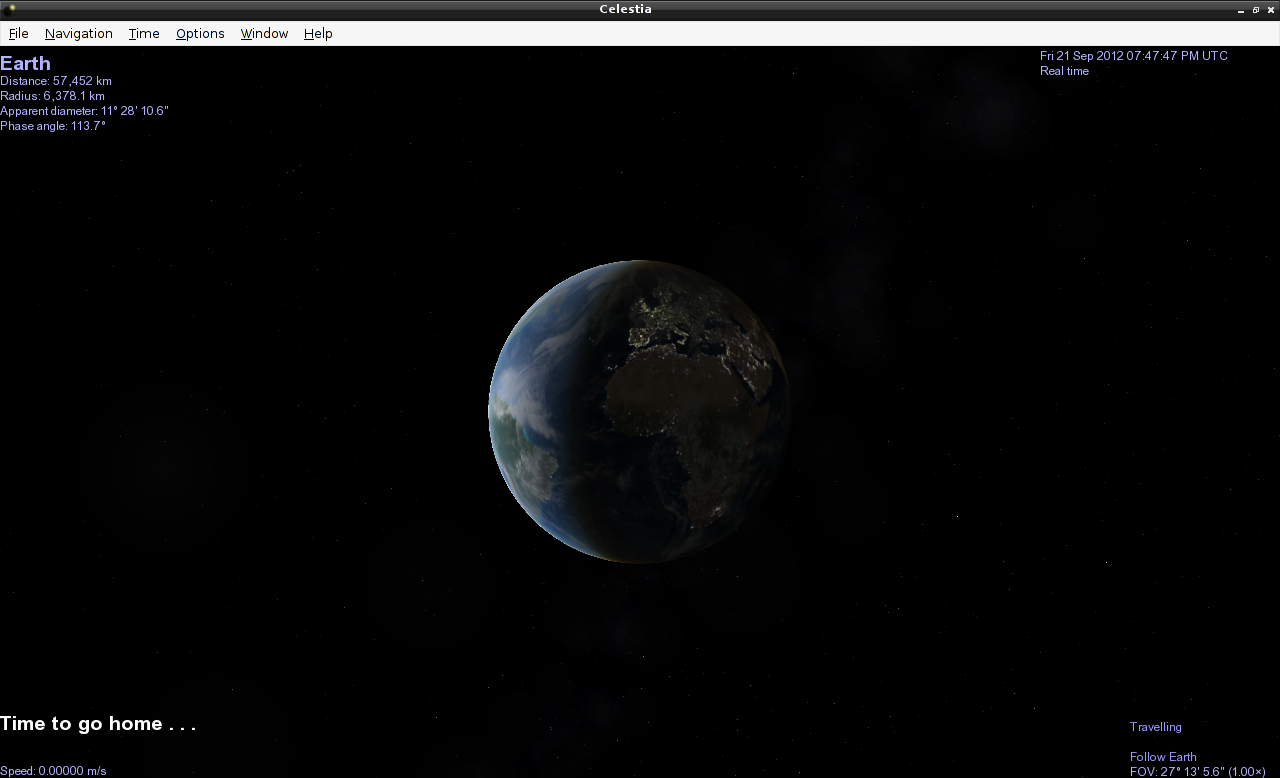
\includegraphics[width=0.5\textwidth]{img/celestia}
    \caption{\emph{Celestia}, vista de la tierra}
    \label{fig:celestia}
\end{figure}
